% !TeX spellcheck = en_US
\section{Introduction}

\subsection {Wupper package}

Approaching a development package bottom up, the Wupper core\footnote{A wupper is a person performing the act of bongelwuppen, the version from the Dutch province of Groningen of the Frisian sport Fierljeppen (canal pole vaulting). \href{https://www.youtube.com/watch?v=Bre8DsQZqSs}{https://www.youtube.com/watch?v=Bre8DsQZqSs}},  is a module of the FELIX firmware and provides an interface for the Direct Memory Acces (DMA) in the Xilinx Virtex-7 FPGA hosted on the VC-709. This FPGA has a PCIe Gen3 hard block integrated in the silicon~\cite{pg023}. With the PCIe Gen3 standard it is possible to reach a theoretical line rate of 8 GT/s; by using 8 lanes, it is therefore possible to reach a theoretical throughput of 64 Gb/s.
The main purpose of Wupper is to handle data transfers from a simple user interface, i.e a FIFO, to and from the host PC memory. The other functionality supported by Wupper is the access to control and monitor registers inside the FPGA, and the surrounding electronics, via a simple register map. Figure~\ref{fig:simplewupperpackage1} below shows a block diagram of the Wupper package. 

\begin{figure}[h]
	\centering
	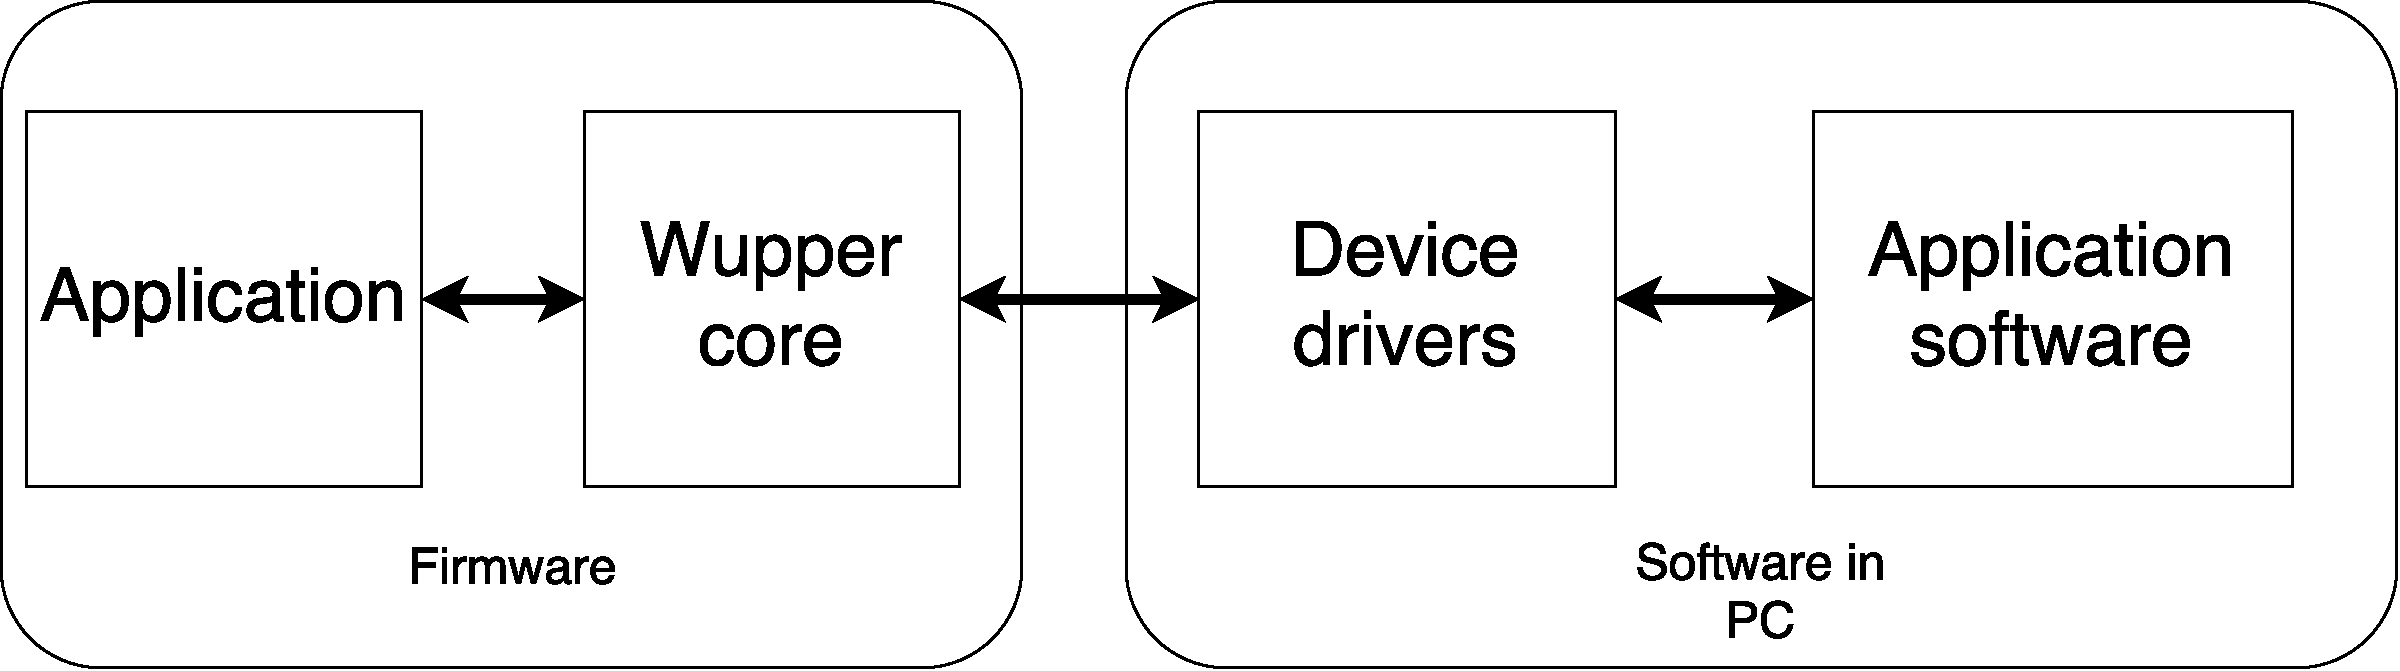
\includegraphics[width = .8 \textwidth]{figures/wupper_package_simple.pdf}	
	\caption{Wupper package overview}
	\label{fig:simplewupperpackage1}
\end{figure}
The Wupper core communicates to the host PC via the Wupper driver and is controlled by a set of, so called, Wupper tools. The Wupper driver through an Application Programming Interface (API) can also communicate to a Wupper Graphical User Interface (GUI). Wupper had been published under the LGPL license on Opencores.org~\cite{opencores}. As the developers firmly believe in the dissemination of knowledge through Open Source. Hence users can freely download, use and learn from the core and possibly provide feedback to further improve Wupper. The outcome of the development is the so called Wupper package: a suite of firmware and software components, which details will be given later in this report. On missing feature of the Wupper core published on OpenCores was a simple yet complete example application to study, test, and benchmark Wupper. To avoid confusion concerning name, a list is created to specify a name and description for all the parts of the Wupper project:

\begin{itemize}
 \item Wupper core: firmware PCIe engine
 \item Wupper driver: software device driver
 \item Wupper tools: software tools to operate the core
 \item Wupper GUI: a simple control and monitor panel
 \item Wupper package: the sum of the above packed for distribution on Open Cores.
\end{itemize}


\newpage
\section{Internship}

\subsection {Goal}
Given the background provided in the previous chapter, my contribution to this project is to develop an example application that checks the health of the core in both directions. The application also checks whether the data that is written into the PC memory is valid. The development contains software (Wupper tools) and an HDL example application.. In addition, a GUI will be developed for the application. Besides those main activities, the device driver and tools developed for Wupper used in the FELIX application has to be ported and tested for the Wupper version published on OpenCores. Appendix B shows the global schedule of the activities I carried out during the development of the application.

\subsection {Topics}
As introduced in the previous paragraph, the aim of this internship is to develop a test application for Wupper. Its purpose is to benchmark the robustness and performance of the Wupper core.
To reach this goal, at first the structure of the Wupper package needs to be understood. This requires grasping how to transfer data using the Wupper core and what is needed for controlling the FPGA using software. Each specific sub-task of the work carried out for this development is detailed in the following sub-paragraphs.


\subsection {Drivers and tools}

%\begin{wrapfigure}[15]{r}{0.4\textwidth}
%	\centering
%	\vspace{-4mm}
%	\includegraphics[width = 0.5 \textwidth]{figures/FELIX_PC.png}	
%	\vspace{-3mm}
%	\caption{Overview of FELIX PC}
%	\label{fig:felixpc}
%\end{wrapfigure}

The drivers and tools are the low level software parts which control the logic of the Wupper core. A set of device drivers are used to: (i) initialize the FPGA PCIe card and control DMA transfers, (ii) perform I/O operations on registers inside the FPGA, (iii) allocate memory buffers in the host PC to be used as landing areas for data transfers.
The Wupper-tools, a collection of tools which is made in the programming languages C and C++, are used to control the logic through the drivers.The Wupper-tools are intended to be a subset of the tools developed for Wupper in the framework of the FELIX project, meaningful for the OpenCores users. The key to implement the Wupper tools is to understand how the original tools work and which parts can be reused.


\subsection {VHDL example application code}
The purpose of the VHDL example application is to show the essentials of the DMA transfer function of Wupper. Prior to the development described in this report, there was only a simple 32-bit counter used to test the data flow in only one direction, i.e. from the FPGA to the PC. Understanding the Wupper core will lead to a renewed version which should transfer 256 bit data with high speed, both in the up and down direction.

\subsection {Developing a GUI}
Prior to this development operating the FPGA card was done via a terminal. There is a certain order to get it working which can be very complicated for the users. The solution is to design a Graphical User Interface (GUI) which can be run on Linux systems.
